% Practice Test 03 — Texas Edition
% Questions: 30 (21 MC + 9 SA)
% Generated by scripts/generate_practice_tests.py

\begin{practiceQuestion}{1-3-q29}{gsa}
\begin{questionText}
The graph shows a proportional relationship. Use the labeled point to find $k$, then determine $y$ when $x = 12$.

\begin{center}
\begin{tikzpicture}[scale=0.6]
  \draw[step=1,gray!20,thin] (0,0) grid (8,8);
  \draw[thick,->] (0,0) -- (8.5,0) node[right]{\small $x$};
  \draw[thick,->] (0,0) -- (0,8.5) node[above]{\small $y$};
  \foreach \x in {2,4,6,8} \draw (\x,0.07) -- (\x,-0.07) node[below]{\tiny \x};
  \foreach \y in {2,4,6,8} \draw (0.07,\y) -- (-0.07,\y) node[left]{\tiny \y};
  \draw[thick,funBlue] (0,0) -- (8,6);
  \fill[funBlue] (0,0) circle (2.5pt);
  \fill[funBlue] (4,3) circle (2.5pt) node[above left]{\small $(4, 3)$};
\end{tikzpicture}
\end{center}
\end{questionText}
\correctAnswer{$k = 0.75$; when $x = 12$, $y = 9$}
\explanation{$k = \frac{3}{4} = 0.75$. Then $y = 0.75 \times 12 = 9$.}
\end{practiceQuestion}

\begin{practiceQuestion}{1-6-q12}{mc}
\begin{questionText}
Store A sells $3$ notebooks for $\$7.50$. Store B sells $5$ notebooks for $\$11.25$. Which store offers the better deal?
\end{questionText}
\choiceA{Store A at $\$2.50$ each}
\choiceB{Store B at $\$2.25$ each}
\choiceC{Store A at $\$2.25$ each}
\choiceD{They cost the same}
\correctAnswer{B}
\explanation{Store A: $7.50 \div 3 = \$2.50$ each. Store B: $11.25 \div 5 = \$2.25$ each. Store B is cheaper.}
\end{practiceQuestion}

\begin{practiceQuestion}{2-1-q11}{mc}
\begin{questionText}
A baker made $120$ cupcakes and sold $90$ of them. What percent of the cupcakes were sold?
\end{questionText}
\choiceA{$60\%$}
\choiceB{$70\%$}
\choiceC{$75\%$}
\choiceD{$80\%$}
\correctAnswer{C}
\explanation{Divide: $90 \div 120 = 0.75 = 75\%$.}
\end{practiceQuestion}

\begin{practiceQuestion}{2-3-q25}{sa}
\begin{questionText}
A store's revenue went from $\$8{,}000$ to $\$6{,}400$. Find the percent decrease.
\end{questionText}
\correctAnswer{$20\%$}
\explanation{Change: $8{,}000 - 6{,}400 = 1{,}600$. Percent decrease: $1{,}600 \div 8{,}000 = 0.20 = 20\%$.}
\end{practiceQuestion}

\begin{practiceQuestion}{2-6-q26}{gmc}
\begin{questionText}
The graph below shows the total amount in a simple interest savings account over time. What is the annual interest rate?

\begin{center}
\begin{tikzpicture}[scale=0.7]
  \draw[thick,->] (0,0) -- (6,0) node[right]{\small Years};
  \draw[thick,->] (0,0) -- (0,6) node[above]{\small Total (\$)};
  \draw[gray!20,thin] (0,0) grid[step=1] (5,5);
  \foreach \x in {0,...,5} {
    \node[below,font=\small] at (\x,0) {$\x$};
  }
  \foreach \y/\lab in {1/200,2/400,3/600,4/800,5/1000} {
    \draw (-0.1,\y) -- (0.1,\y) node[left,font=\small,xshift=-2pt] {\lab};
  }
  % Points: P = 800, r = 5%, so total = 800 + 40t
  % t=0: 800, t=1: 840, t=2: 880, t=3: 920, t=4: 960, t=5: 1000
  \filldraw[funBlue] (0,4) circle (3pt);
  \filldraw[funBlue] (1,4.2) circle (3pt);
  \filldraw[funBlue] (2,4.4) circle (3pt);
  \filldraw[funBlue] (3,4.6) circle (3pt);
  \filldraw[funBlue] (4,4.8) circle (3pt);
  \filldraw[funBlue] (5,5) circle (3pt);
  \draw[thick,funBlue] (0,4) -- (1,4.2) -- (2,4.4) -- (3,4.6) -- (4,4.8) -- (5,5);
  \node[right,font=\small] at (0.1,4) {$\$800$};
  \node[right,font=\small] at (5.1,5) {$\$1{,}000$};
\end{tikzpicture}
\end{center}
\end{questionText}
\choiceA{$4\%$}
\choiceB{$5\%$}
\choiceC{$8\%$}
\choiceD{$10\%$}
\correctAnswer{B}
\explanation{Principal: $\$800$. After $5$ years: $\$1{,}000$. Interest: $1{,}000 - 800 = \$200$. Rate: $200 = 800 \times r \times 5$ → $r = 200 \div 4{,}000 = 0.05 = 5\%$.}
\end{practiceQuestion}

\begin{practiceQuestion}{2-8-q18}{mc}
\begin{questionText}
Why is it important to pay your credit card bill on time?
\end{questionText}
\choiceA{To earn more interest from the credit card company}
\choiceB{To avoid paying extra interest charges}
\choiceC{To increase the card's interest rate}
\choiceD{To close your bank account}
\correctAnswer{B}
\explanation{Paying on time avoids interest charges. Late payments mean you pay more for the same purchase.}
\end{practiceQuestion}

\begin{practiceQuestion}{2-9-q26}{gmc}
\begin{questionText}
The circle graph shows how a student spends her monthly income of $\$800$. How much does she spend on food?

\begin{center}
\begin{tikzpicture}[scale=1.2]
  % Pie chart
  \fill[funBlue!60] (0,0) -- (90:1.5) arc (90:198:1.5) -- cycle;
  \fill[funRed!60] (0,0) -- (198:1.5) arc (198:306:1.5) -- cycle;
  \fill[green!50!black] (0,0) -- (306:1.5) arc (306:378:1.5) -- cycle;
  \fill[orange!60] (0,0) -- (18:1.5) arc (18:90:1.5) -- cycle;
  \draw[thick] (0,0) circle (1.5);
  % Labels
  \node at (144:1) {\footnotesize Rent};
  \node at (144:0.55) {\footnotesize $30\%$};
  \node at (252:1) {\footnotesize Food};
  \node at (252:0.55) {\footnotesize $30\%$};
  \node at (342:1) {\footnotesize Fun};
  \node at (342:0.55) {\footnotesize $20\%$};
  \node at (54:1) {\footnotesize Save};
  \node at (54:0.55) {\footnotesize $20\%$};
\end{tikzpicture}
\end{center}
\end{questionText}
\choiceA{$\$160$}
\choiceB{$\$200$}
\choiceC{$\$240$}
\choiceD{$\$300$}
\correctAnswer{C}
\explanation{Food is $30\%$ of $\$800$: $800 \times 0.30 = \$240$.}
\end{practiceQuestion}

\begin{practiceQuestion}{2-10-q19}{sa}
\begin{questionText}
Deposit $\$600$ at $5\%$ compounded yearly. Find the total after $2$ years.
\end{questionText}
\correctAnswer{$\$661.50$}
\explanation{Year 1: $600 \times 1.05 = \$630$. Year 2: $630 \times 1.05 = \$661.50$.}
\end{practiceQuestion}

\begin{practiceQuestion}{4-1-q12}{mc}
\begin{questionText}
Evaluate $\frac{3x + 1}{2}$ when $x = 5$.
\end{questionText}
\choiceA{$7$}
\choiceB{$8$}
\choiceC{$8.5$}
\choiceD{$7.5$}
\correctAnswer{B}
\explanation{Substitute: $\frac{3(5) + 1}{2} = \frac{15 + 1}{2} = \frac{16}{2} = 8$.}
\end{practiceQuestion}

\begin{practiceQuestion}{4-2-q11}{mc}
\begin{questionText}
How many terms are in the simplified form of $8b - 3 + 2b + 5 - b$?
\end{questionText}
\choiceA{$5$}
\choiceB{$3$}
\choiceC{$2$}
\choiceD{$1$}
\correctAnswer{C}
\explanation{Combine variable terms: $8b + 2b - b = 9b$. Combine constants: $-3 + 5 = 2$. Simplified: $9b + 2$, which has $2$ terms.}
\end{practiceQuestion}

\begin{practiceQuestion}{5-3-q16}{mc}
\begin{questionText}
Solve $8(x + 1) = 48$.
\end{questionText}
\choiceA{$x = 5$}
\choiceB{$x = 6$}
\choiceC{$x = 7$}
\choiceD{$x = \dfrac{47}{8}$}
\correctAnswer{A}
\explanation{Divide by $8$: $x + 1 = 6$. Subtract $1$: $x = 5$. Check: $8(5 + 1) = 8(6) = 48$ \checkmark.}
\end{practiceQuestion}

\begin{practiceQuestion}{5-4-q13}{mc}
\begin{questionText}
A shirt is on sale for $\dfrac{2}{3}$ of its original price. After using a $\$5$ coupon, you pay $\$15$. What equation finds the original price $p$?
\end{questionText}
\choiceA{$\dfrac{2}{3}p + 5 = 15$}
\choiceB{$p - \dfrac{2}{3} - 5 = 15$}
\choiceC{$\dfrac{2}{3}p - 5 = 15$}
\choiceD{$\dfrac{2}{3}(p - 5) = 15$}
\correctAnswer{C}
\explanation{Sale price is $\frac{2}{3}p$. After the $\$5$ coupon: $\frac{2}{3}p - 5 = 15$.}
\end{practiceQuestion}

\begin{practiceQuestion}{5-5-q02}{mc}
\begin{questionText}
Solve $-3n + 6 \leq 0$.
\end{questionText}
\choiceA{$n \leq 2$}
\choiceB{$n \leq -2$}
\choiceC{$n \geq 2$}
\choiceD{$n \geq -2$}
\correctAnswer{C}
\explanation{Subtract $6$: $-3n \leq -6$. Divide by $-3$ and flip the sign: $n \geq 2$.}
\end{practiceQuestion}

\begin{practiceQuestion}{5-6-q05}{mc}
\begin{questionText}
Which inequality is shown by a closed circle at $7$ with shading to the left?
\end{questionText}
\choiceA{$x > 7$}
\choiceB{$x < 7$}
\choiceC{$x \geq 7$}
\choiceD{$x \leq 7$}
\correctAnswer{D}
\explanation{Closed circle means the endpoint is included, shading left means less than or equal to: $x \leq 7$.}
\end{practiceQuestion}

\begin{practiceQuestion}{6-2-q27}{gmc}
\begin{questionText}
The two rectangles below represent the same room drawn at two different scales. The original uses $1$ cm $= 6$ m. What scale does the new drawing use?

\begin{center}
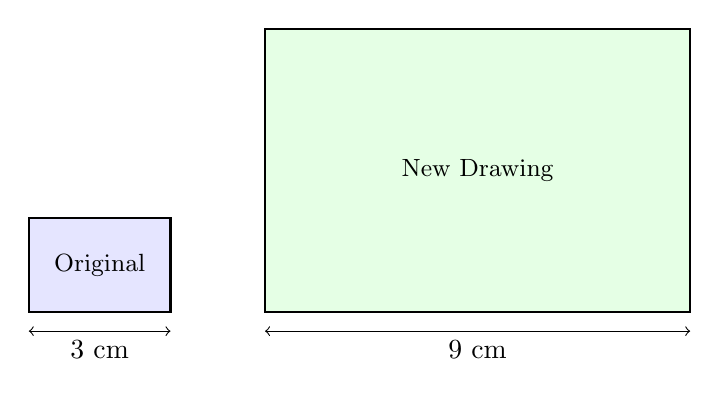
\begin{tikzpicture}[scale=0.6]
  % Original
  \draw[thick,fill=blue!10] (0,0) rectangle (3,2);
  \node at (1.5,1) {\small Original};
  \draw[<->] (0,-0.4) -- (3,-0.4);
  \node[below] at (1.5,-0.4) {$3$ cm};
  % New
  \draw[thick,fill=green!10] (5,0) rectangle (14,6);
  \node at (9.5,3) {\small New Drawing};
  \draw[<->] (5,-0.4) -- (14,-0.4);
  \node[below] at (9.5,-0.4) {$9$ cm};
\end{tikzpicture}
\end{center}
\end{questionText}
\choiceA{$1$ cm $= 2$ m}
\choiceB{$1$ cm $= 3$ m}
\choiceC{$1$ cm $= 6$ m}
\choiceD{$1$ cm $= 18$ m}
\correctAnswer{A}
\explanation{Scale ratio: $9 \div 3 = 3$. The new drawing is $3$ times bigger. Actual length: $3 \times 6 = 18$ m. New scale: $18 \div 9 = 2$ m per cm.}
\end{practiceQuestion}

\begin{practiceQuestion}{6-3-q20}{sa}
\begin{questionText}
A triangle has two sides of length $8$ cm and $12$ cm. What is the range of possible lengths for the third side?
\end{questionText}
\correctAnswer{Greater than $4$ cm and less than $20$ cm}
\explanation{By the triangle inequality: $12 - 8 < \text{third side} < 12 + 8$, so $4 < \text{third side} < 20$.}
\end{practiceQuestion}

\begin{practiceQuestion}{6-4-q25}{sa}
\begin{questionText}
A triangle has angles $60°$, $60°$, and $60°$, and one side measures $10$ cm. How many triangles can be drawn?
\end{questionText}
\correctAnswer{Exactly one}
\explanation{AAA alone gives many, but specifying a side length fixes the size. A triangle with all $60°$ angles is equilateral, so all sides are $10$ cm. Exactly one triangle.}
\end{practiceQuestion}

\begin{practiceQuestion}{6-5-q01}{mc}
\begin{questionText}
You slice a rectangular prism with a cut parallel to its base. What shape is the cross-section?
\end{questionText}
\choiceA{Triangle}
\choiceB{Circle}
\choiceC{Rectangle}
\choiceD{Pentagon}
\correctAnswer{C}
\explanation{A horizontal cut parallel to the base of a rectangular prism produces a rectangle the same shape as the base.}
\end{practiceQuestion}

\begin{practiceQuestion}{6-8-q05}{mc}
\begin{questionText}
A flagpole casts a $24$-ft shadow. At the same time, a $6$-ft person casts an $8$-ft shadow. How tall is the flagpole?
\end{questionText}
\choiceA{$12$ ft}
\choiceB{$18$ ft}
\choiceC{$32$ ft}
\choiceD{$20$ ft}
\correctAnswer{B}
\explanation{Set up: $\frac{6}{8} = \frac{h}{24}$. Cross-multiply: $8h = 144$. Divide: $h = 18$ ft.}
\end{practiceQuestion}

\begin{practiceQuestion}{7-4-q06}{mc}
\begin{questionText}
An L-shaped room can be split into a $10$ ft by $8$ ft rectangle and a $4$ ft by $6$ ft rectangle. What is the total floor area?
\end{questionText}
\choiceA{$56$ ft$^2$}
\choiceB{$80$ ft$^2$}
\choiceC{$104$ ft$^2$}
\choiceD{$128$ ft$^2$}
\correctAnswer{C}
\explanation{$10 \times 8 = 80$ ft$^2$. $4 \times 6 = 24$ ft$^2$. Total: $80 + 24 = 104$ ft$^2$.}
\end{practiceQuestion}

\begin{practiceQuestion}{7-5-q30}{gsa}
\begin{questionText}
A box without a lid is shown below. What is the total surface area (including the bottom but NOT the top)?

\begin{center}
\begin{tikzpicture}[scale=0.4]
  % Front face
  \draw[thick,funBlue,fill=funBlue!10] (0,0) -- (8,0) -- (8,5) -- (0,5) -- cycle;
  % Top (open — dashed)
  \draw[thick,dashed,gray] (0,5) -- (3,7) -- (11,7) -- (8,5);
  % Right face
  \draw[thick,funBlue,fill=funBlue!15] (8,0) -- (11,2) -- (11,7) -- (8,5) -- cycle;
  % Labels
  \draw[thick,funRed,<->] (0,-0.7) -- (8,-0.7);
  \node[below,funRed] at (4,-0.7) {$8$ cm};
  \draw[thick,funRed,<->] (11.5,2) -- (11.5,7);
  \node[right,funRed] at (11.5,4.5) {$5$ cm};
  \draw[thick,funRed,<->] (8,-0.7) -- (11,-0.7+2);
  \node[below right,funRed] at (9.5,0) {$3$ cm};
\end{tikzpicture}
\end{center}
\end{questionText}
\correctAnswer{$134$ cm$^2$}
\explanation{Bottom: $8 \times 3 = 24$ cm$^2$. Front and Back: $2(8 \times 5) = 80$ cm$^2$. Two sides: $2(3 \times 5) = 30$ cm$^2$. Total (no top): $24 + 80 + 30 = 134$ cm$^2$.}
\end{practiceQuestion}

\begin{practiceQuestion}{7-6-q14}{mc}
\begin{questionText}
A rectangular prism is $8$ in by $5$ in by $4$ in. Another is $10$ in by $4$ in by $4$ in. Which has more volume and by how much?
\end{questionText}
\choiceA{First prism, by $10$ in$^3$}
\choiceB{Second prism, by $10$ in$^3$}
\choiceC{First prism, by $20$ in$^3$}
\choiceD{They have the same volume}
\correctAnswer{D}
\explanation{First: $8 \times 5 \times 4 = 160$ in$^3$. Second: $10 \times 4 \times 4 = 160$ in$^3$. They have the same volume.}
\end{practiceQuestion}

\begin{practiceQuestion}{8-1-q02}{mc}
\begin{questionText}
A researcher wants to know the average height of seventh graders in a state. She measures the heights of $100$ seventh graders from different schools. What is the sample?
\end{questionText}
\choiceA{All seventh graders in the state}
\choiceB{All students in the schools she visited}
\choiceC{The $100$ seventh graders she measured}
\choiceD{The tallest seventh graders}
\correctAnswer{C}
\explanation{The sample is the smaller group chosen from the population — the $100$ students measured.}
\end{practiceQuestion}

\begin{practiceQuestion}{8-2-q24}{sa}
\begin{questionText}
A random sample of $25$ watermelons has a mean weight of $8$ kg. Predict the total weight of $500$ watermelons from the same farm.
\end{questionText}
\correctAnswer{$4{,}000$ kg}
\explanation{$500 \times 8 = 4{,}000$ kg.}
\end{practiceQuestion}

\begin{practiceQuestion}{8-4-q19}{sa}
\begin{questionText}
Data: $30, 35, 40, 45, 50$. Find the mean and range.
\end{questionText}
\correctAnswer{Mean $= 40$; Range $= 20$}
\explanation{Mean: $\frac{30+35+40+45+50}{5} = \frac{200}{5} = 40$. Range: $50 - 30 = 20$.}
\end{practiceQuestion}

\begin{practiceQuestion}{8-5-q04}{mc}
\begin{questionText}
Data: $12, 15, 21, 23, 27, 30, 35$. In a stem-and-leaf plot, what are the stems?
\end{questionText}
\choiceA{$1, 2, 3$}
\choiceB{$2, 5, 1, 3, 7, 0, 5$}
\choiceC{$12, 15, 21, 23, 27, 30, 35$}
\choiceD{$10, 20, 30$}
\correctAnswer{A}
\explanation{The stems are the tens digits: $1$ (for $12, 15$), $2$ (for $21, 23, 27$), $3$ (for $30, 35$).}
\end{practiceQuestion}

\begin{practiceQuestion}{8-6-q13}{mc}
\begin{questionText}
Which is NOT a good use of a circle graph?
\end{questionText}
\choiceA{Showing the breakdown of a budget}
\choiceB{Showing parts of a whole survey result}
\choiceC{Comparing temperatures over time}
\choiceD{Showing how students spend their time}
\correctAnswer{C}
\explanation{Circle graphs show parts of a whole. For data that changes over time, a line graph is more appropriate.}
\end{practiceQuestion}

\begin{practiceQuestion}{9-4-q27}{gmc}
\begin{questionText}
The table shows a probability model for a spinner. The spinner is spun $100$ times and the results are shown. Does the observed data support the model?

\begin{center}
\begin{tabular}{|c|c|c|}
\hline
\textbf{Color} & \textbf{Model $P$} & \textbf{Observed Frequency} \\
\hline
Red & $0.40$ & $38$ \\
\hline
Blue & $0.35$ & $36$ \\
\hline
Yellow & $0.25$ & $26$ \\
\hline
\end{tabular}
\end{center}
\end{questionText}
\choiceA{No, the data is very different from the model}
\choiceB{Yes, the observed frequencies are close to the predicted values}
\choiceC{No, because Red appeared fewer times than predicted}
\choiceD{The model cannot be checked with only $100$ spins}
\correctAnswer{B}
\explanation{Predicted: Red $= 40$, Blue $= 35$, Yellow $= 25$. Observed: $38$, $36$, $26$. These are close, supporting the model.}
\end{practiceQuestion}

\begin{practiceQuestion}{9-6-q01}{mc}
\begin{questionText}
What is the probability of flipping two coins and getting heads on both?
\end{questionText}
\choiceA{$\frac{1}{2}$}
\choiceB{$\frac{1}{3}$}
\choiceC{$\frac{1}{4}$}
\choiceD{$\frac{3}{4}$}
\correctAnswer{C}
\explanation{Sample space: HH, HT, TH, TT ($4$ outcomes). Only HH is heads-heads. $P = \frac{1}{4}$.}
\end{practiceQuestion}

\begin{practiceQuestion}{9-7-q20}{sa}
\begin{questionText}
You roll a die $90$ times to simulate a $\frac{1}{6}$ probability event. How many times do you expect the event to occur?
\end{questionText}
\correctAnswer{$15$}
\explanation{$90 \times \frac{1}{6} = 15$.}
\end{practiceQuestion}
